% !TEX root = thesis.tex
\chapter{Facebookの顔画像認識と深層学習技術}
この章では、深層学習を画像認識の問題に適用した応用例を挙げる。\par
ソーシャルメディアのユーザ属性を推定することは、マーケティングやネット広告の最適化において有益である。ここでは、公開プロフィールの一種であるプロフィール画像に着目する。入力となるプロフィール画像と、推定する目標であるユーザ属性のセットを用いて、深層学習を行わせることで、より精度の高いユーザ属性推定を目指す。

\section{背景}
ソーシャルメディアのユーザプロフィールから、そのユーザの属性を推定するためのアルゴリズムが求められている。\\
マーケティングや、ネット広告の最適化などに応用可能で、ビジネス面において大きな貢献が期待できる。\par
ユーザ属性の推定元としては、名前 / 日記 / ツイートなどのテキストデータ、プロフィールなどの画像、友達関係などが挙げられる。\cite{pennacchiotti2011a-machine}

テキストデータは量が豊富だが、ソーシャルメディアの種類によっては、「友達のみ公開」などの設定がされている。ネット広告を載せる企業の視点から見ると、常に自由にアクセスできるとは限らない。\\

一方プロフィール画像は、ほぼ全てのソーシャルメディアにおいて、全員に公開されている。ネット広告企業からでも、必ずチェックできる。\\

画像からユーザ属性を推定できれば、より多くの場面で、効率の良いマーケティングが可能になる。これはテキストベースの方法にはない、大きなメリットである。\\

しかし、プロフィール画像を元データとした研究はまだメジャーではない。\\
最終的に、ソーシャルメディアのプロフィール画像が与えられれば、ユーザ属性を推定できる状態を目指す。\\
その過程として、今回の領域プロジェクトでは、「Facebook」より「プロフィール顔画像」に限定してのユーザ推定を試みる。\par

\begin{figure}[tbp]
 \begin{center}
  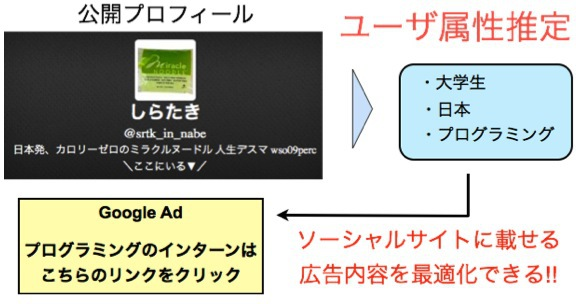
\includegraphics[width=100mm]{img/c7/prof2prop}
 \end{center}
 \caption{ユーザ属性推定の必要性}
 \label{c7_prof2prop}
\end{figure}

公開プロフィールからユーザ属性を推定するというアプローチによる過去の研究としては、Twitterのプロフィールやツイート内容、フォロー関係などから、ユーザ属性を割り出したものがある\cite{pennacchiotti2011a-machine}。この研究では、「スターバックスが好きか」「支持政党は民主党と共和党のどちらか」「どの民族 (ethnicity)に属しているか」といった情報を推定している。\par
なお、この研究においては、プロフィール写真はユーザ属性を推定する参考になりにくいとされている。彼らに拠れば、ソーシャルメディアのユーザーは、必ずしもプロフィール画像にユー
ザ本人の画像を用いるわけではない。むしろ、有名人の画像が使われていて、本人の属性推定においてノイズとなってしまうケースもある。\par
また、別の研究\cite{mislove2011understanding}では、Twitterのデータより、Twitterのユーザ構成の傾向について、基本的なデータを収集している。具体的には、位置情報より居住地の傾向を、first nameから性別の傾向を、last nameから宗教の傾向を割り出している。なお、この研究でもプロフィール画像データは用いられていなかった。\par
H. Andrew Schwartzらは、公開プロフィールという制限こそ課していないが、75000名のユーザ有志より、7000万個の単語や言葉、話題の例を収集して分析にかけ、同時に収集した年齢・性別・性格テストのデータとの相関性を学習させることや、言葉遣いからこれらのユーザ属性を精度良く推測させることに成功した\cite{schwartz2013personality}。彼らは、年代や性格ごとに特徴的な言葉遣いを可視化しており、可視化の結果はウェブサイトにて見ることができる\footnote{\url{http://wwbp.org/}}。

\begin{figure}[tbp]
 \begin{center}
  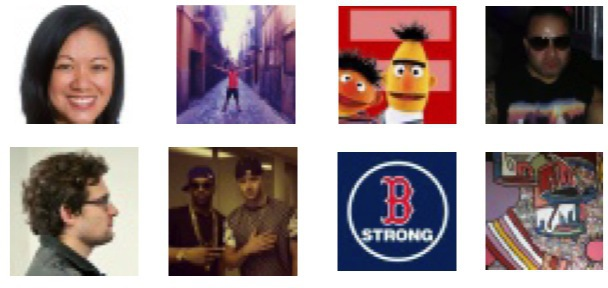
\includegraphics[width=100mm]{img/c7/pic_sample}
 \end{center}
 \caption{Facebookにおけるプロフィール画像の例}
 \label{c7_pic_sample}
\end{figure}

\section{ソーシャルメディアにおける、プロフィール画像}
図\ref{c7_pic_sample}に、実際にFacebookにて利用されているプロフィール画像の例を挙げる。これはごく一部の例であるが、これらを見るだけでも、以下の障害となりそうな点が考えられる。
\begin{itemize}
\item \textbf{人間が写っているとは限らない。}人気キャラクターやブランドのロゴ、絵画が含まれている。入力データのバリエーションが増えることで、学習が難しくなることが予想される。
\item \textbf{2人以上の人間が映っていることがある。}例えば、カップルの写真やクラスの集合写真がプロフィール画像として使われていたとき、誰がユーザ本人であるかを推定するのは極めて困難だと想像できる。
\item \textbf{本人の画像かどうかわからない。}先述した研究\cite{pennacchiotti2011a-machine}でも述べられている通り、少なくとも画像自体の中に、本人である証拠はない。有名人に関しては、有名人の顔写真のデータベースを別途作成することで対応できる可能性があるが、あまり知られていない他人の写真だった場合、対処は難しい。
\item \textbf{顔が鮮明でないことがある。}例え本人が写っていても、顔の拡大写真ではなく、全身が映されていて、顔がぼやけてしまっていることがある。
\end{itemize}
以上をまとめると、「プロフィール画像=ユーザの顔」という前提が成り立たないという問題点が浮き彫りになる。この前提が成り立たない場合、「画像 = ユーザの顔→ユーザの年齢や性別」という一段階の推論ではなく、「画像→本人か?→本人でなかったら、誰の容姿なのか、またはキャラクターやブランドなのか→その有名人やキャラクターを好むユーザは、どのような年齢や性別が多いか?」という多段階の推論が必要となり、学習難易度が高くなると考えられる。\par
今回は、

\section{提案手法}
図\ref{c7_proposal}は、今回の提案手法を表している。提案手法は、次の3ステップより成る。
\begin{enumerate}
\item \textbf{ソーシャルメディアより、プロフィール画像を得る。}この方法はソーシャルメディア毎に大きく異なるが、各メディアが提供しているAPIや、閲覧者用のウェブページより、様々なユーザのプロフィール画像を取得する。また、このときユーザ属性の教師データを取得できる場合もある。
\item \textbf{プロフィール画像を、ベクトルデータに変換する。}基本的には、画像の各画素値そのものを、入力ベクトルとして使用する。これは、可能な限り取得したままのデータを加工せずに入力することで、素性の採り方自体を学習できる深層学習の特徴を活かせるからである。ただし,対象データによっては,画像の特徴量を付加することで精度が上昇する\cite{ciresan2012multi-column}ことが知られており、工夫の余地もある。
\item \textbf{ベクトルデータから、分類器を使って、ユーザ属性を識別する。}機械学習により、画像のベクトルデータからユーザ属性を推定できるような、クラス識別モデルを取得する。深層学習が応用されるのは、この部分である。
\end{enumerate}


\begin{figure}[tbp]
 \begin{center}
  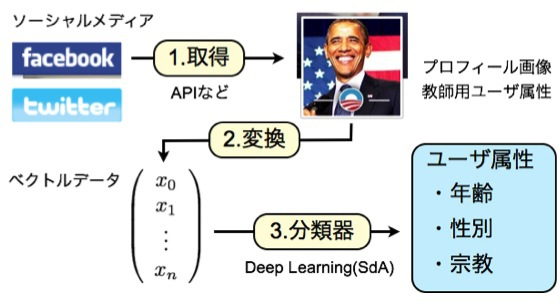
\includegraphics[width=100mm]{img/c7/proposal}
 \end{center}
 \caption{提案手法}
 \label{c7_proposal}
\end{figure}

\section{問題設定と、実験方法の詳細}
今回の実験では、ソーシャルメディアのプロフィール画像からユーザ属性を推定する例として、Facebookのプロフィール画像のうち、人間の顔画像を1つだけ含んでいるものを対象として、ユーザの性別を推定出来るかどうか、学習を行わせた。以下に、実験方法の詳細を記す。
\subsection{画像の取得と加工}
Facebookの公開APIを用いて、サイズ200x200(px)のプロフィール画像を11028件取得した。画像と同時に、ユーザの性別データも収集した。\par
取得した画像からは、条件に合わないものを除外すると同時に、顔の特徴が失われない範囲で、学習速度を上げるための前処理を施した。まず、各画像をRGBカラーからグレースケールに変換した。次に、人間の顔画像がちょうど1人分入っているかどうか、判定を行った。これには画像処理ライブラリのOpenCVに含まれている、顔画像識別のプログラム\footnote{\url{http://docs.opencv.org/trunk/modules/objdetect/doc/cascade_classification.html}}を用いた。識別器には、LBP Cascade法\cite{liao2007learning}を使った。判別の結果、サイズ20x20[px]以上で正面を向いた1人分の顔画像が検出できた場合のみ、その画像を使用した(図\ref{c7_pic_sample})。さらに、検出した顔領域が中心で一定のサイズを占めるように、画像を切り抜き、30x30[px]に解像度を落とした。また、より画像の特徴がわかりやすくなって学習が進むよう、色調を平均化補正し、コントラストが際立つようにした。\par
以上の行程により、男性2180件、女性1566件、計3746件の画像データ及び、対応する性別のデータが集まった。
\subsection{ベクトルデータへの変換}
平面的な広がりを持つ画像データから、画素値[0.0-1.0)を要素とする900次元のベクトルデータへの変換を施した。画像の各画素と、ベクトルの順番の関係は、図\ref{c7_conv}のようになっており、この図における画素の番号と、ベクトルの要素番号が対応している。
\subsection{ユーザの分類}
入力がここまでの変換で得たベクトルデータ、出力がユーザの性別の、クラス分類問題として考える。
分類器に学習を行わせ、ユーザを精度よく分類することを目指す。学習モデルとしては、深層ニューラルネットワークの一種である積層雑音除去自己符号器(以下SDA)と、従来手法としてのサポートベクターマシン(以下SVM)の2つを用いた。\par
SDAの実装には,ウェブサイトDeep Learning Tutorial\footnote{\url{http://www.deeplearning.net/tutorial}}にて提供されているものを用いた。corruption rateは30\%とした。また、SVMの実装には、専用ライブラリのLIBSVM\footnote{\url{http://www.csie.ntu.edu.tw/~cjlin/LIBSVM/}}を用いた。
\par

\begin{figure}[tbp]
 \begin{center}
  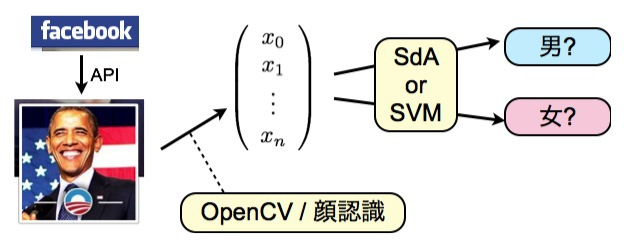
\includegraphics[width=80mm]{img/c7/expr}
 \end{center}
 \caption{今回の実験の模式図}
 \label{c7_expr}
\end{figure}

\begin{figure}[tbp]
 \begin{center}
  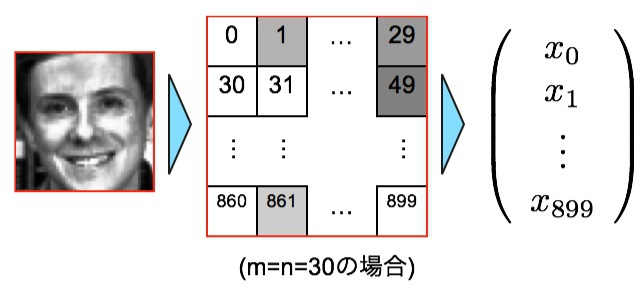
\includegraphics[width=80mm]{img/c7/conv}
 \end{center}
 \caption{実験で使った、画像から入力ベクトルへの変換方法}
 \label{c7_conv}
\end{figure}

\begin{figure}[tbp]
 \begin{center}
  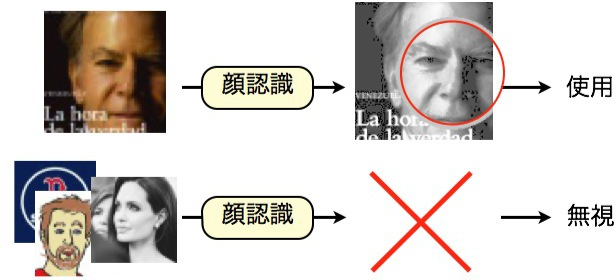
\includegraphics[width=80mm]{img/c7/pic_judge}
 \end{center}
 \caption{プロフィール画像からの顔画像抽出方法}
 \label{c7_pic_judge}
\end{figure}

\section{結果}
分類精度は、表\ref{c7_fb_result}の通りとなった。深層学習のSDAの方が、少し精度が低い結果となってしまった。\par
\begin{table}[tbp]
 \begin{center}
  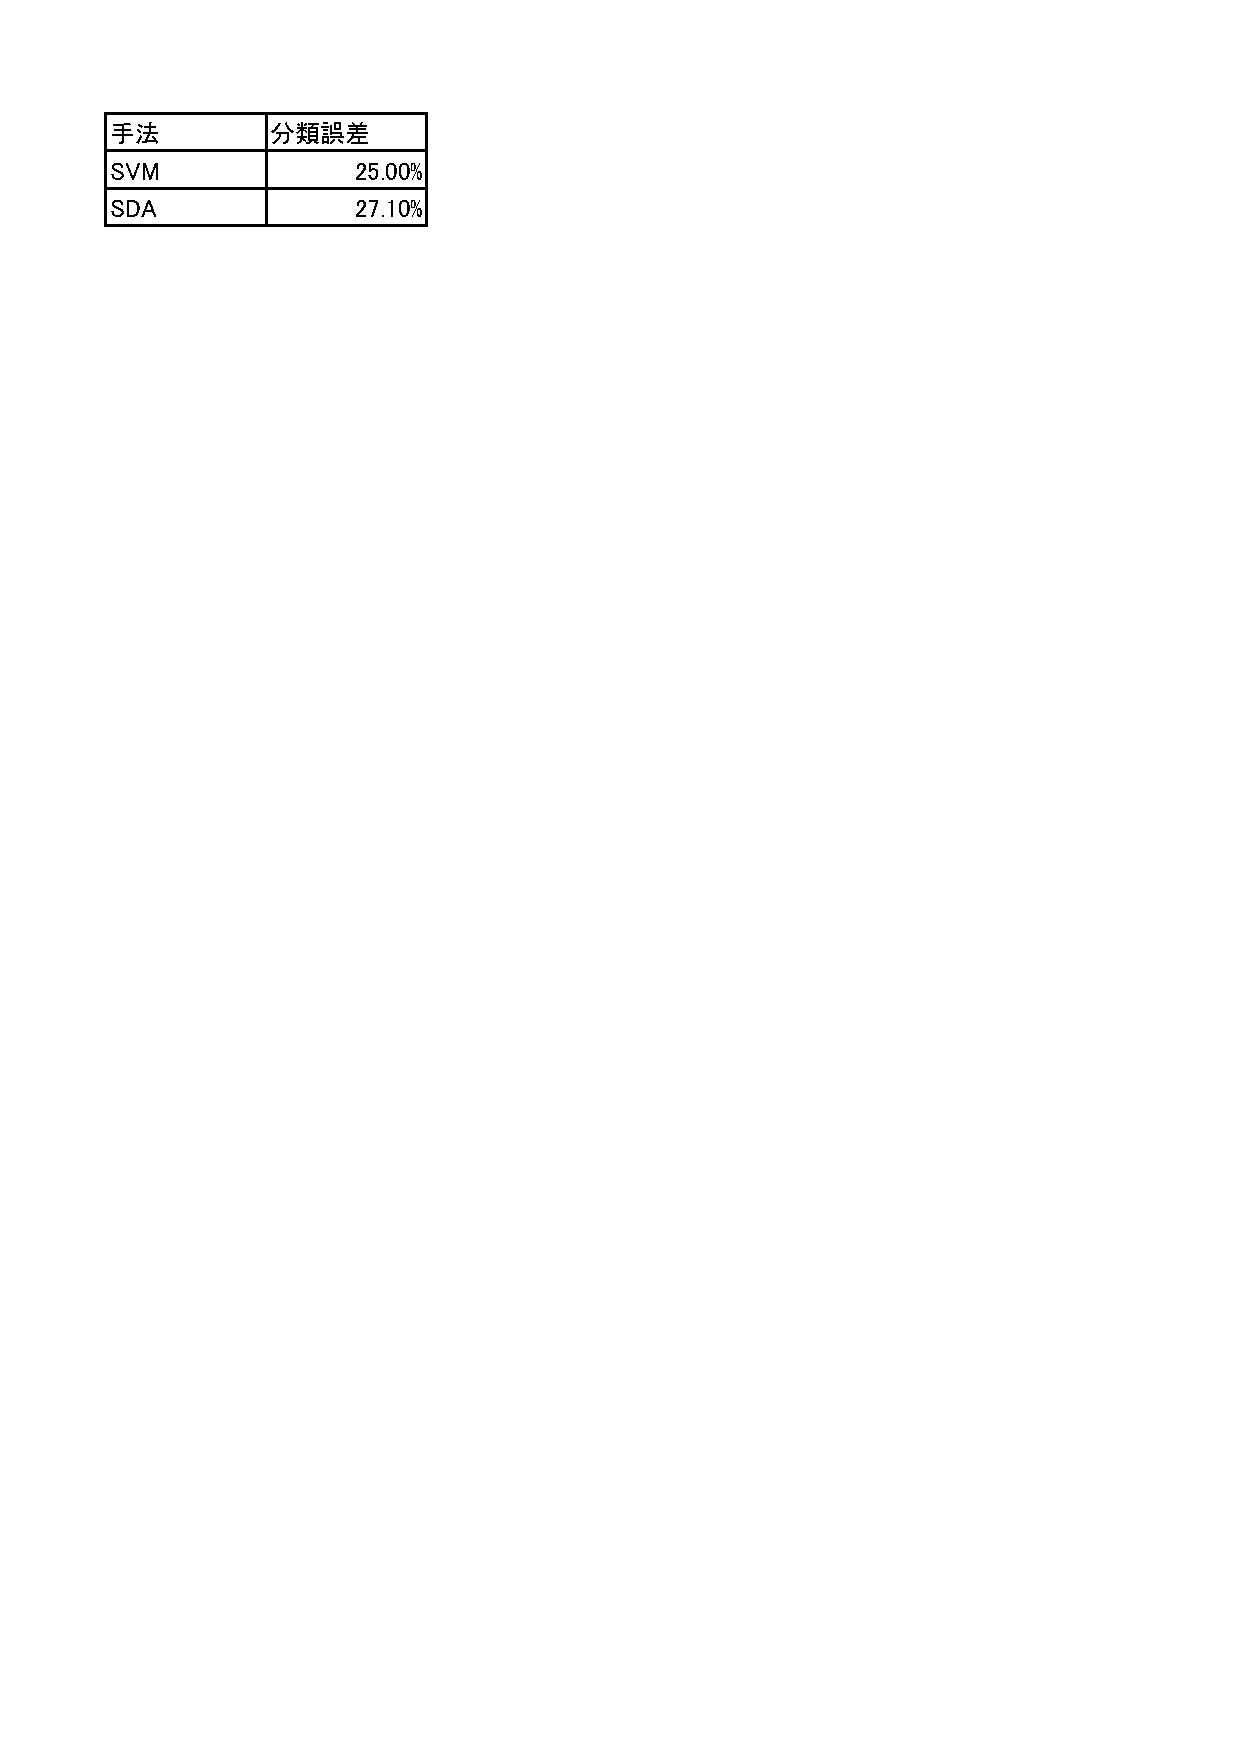
\includegraphics[width=60mm]{img/c7/fb_result}
 \end{center}
 \caption{Facebook顔画像の分類結果}
 \label{c7_fb_result}
\end{table}
なお、図\ref{c7_フィルタ}に、今回の実験でSDAが学習した、1レイヤー目のフィルターを示す。SDAは精度こそ僅かに劣っているものの、今回の方法でも顔を学習すること自体には成功していることがわかる。

\begin{figure}[tbp]
 \begin{center}
  \includegraphics[width=100mm]{img/c7/フィルタ}
 \end{center}
 \caption{実験で学習されたフィルター}
 \label{c7_フィルタ}
\end{figure}

\section{考察}
\subsection{全体の結果のまとめ}
この章の実験では、ソーシャルメディアのユーザ属性推定において、プロフィール画像からの推定手法を模索した。実験の結果、SDA、SVM共に、Facebookのユーザプロフィールにて1人分の顔画像が使われているという条件ならば、ある程度ユーザの性別を識別できることがわかった。\par
\subsection{SDAにて良い精度が出なかった理由の考察}
識別自体にはある程度成功したとはいえ、本来画像認識や多段階の推論で効果を発揮すると思われる深層学習を使用したにも関わらず、従来から用いられている単純なSVMによる精度を上回ることが出来なかった。この理由はわかっていないが、考えられることとして、まず実験で用意したデータ数の不足や偏りが考えられる。例えば、深層学習全般が大きな成果を挙げているMNISTのデータセットには、全体で70000のデータが用意されている。また、CIFAR10でも60000件のデータが利用可能である。比べて、今回用意できたデータは3746件のみであり、男性と女性のデータ数には1.3倍ほどの開きがあった。このデータの不足と偏りが、学習傾向に歪みを与えてしまった可能性がある。\par
また、隠れレイヤー数、レイヤー内ユニット数など、学習モデルを形成する様々なハイパーパラメータの調整を行うことで、学習制度を向上させることができる可能性がある。SVMの場合、grid searchと呼ばれる方法によってパラメータを調整している。しかし、この方法はハイパーパラメータが増加するにつれて指数関数的にかかる時間が増大してしまう。パラメータが1〜3個程度で済むSVMでは有効な方法だが、パラメータ数が非常に多いSDAや他の深層学習の方法では、現実的ではない。ハイパーパラメータを自動的に調整する方法が必要である。\par
ハイパーパラメータを調整する方法としては、\cite{bengio2012practical}にて、Grid Searchによってしらみつぶしに探すよりも、Random Searchを用いた方が効率が良いと述べられており、今後実験を行う際には参考にしようと思う。また、実験用ビルドシステムを併用することも効果的だと思われる\footnote{\url{https://github.com/pfi/maf}}。

\subsection{今後の発展について}
今回の実験では、まず最も確実性の高いところから検証するということで、単体の顔プロフィール画像のみを識別のターゲットとした。しかし、キャラクターやブランドロゴなどの非実写アイコンや、人間の横顔、複数人が映った画像からでもユーザ属性が推定できれば、より応用での確実性が増す。性別だけでなく、ユーザの好みや交友関係の傾向も推測できれば、これも貴重な情報となる。人間の行動や思考は、テキストだけでなく、ファッションや交友関係など非言語的な特徴にも顕れる。こういった情報も学習できるようになれば、システムの利用価値が高くなっていくと思われる。\par
Facebookは、本人画像の使用率が比較的高いコミュニティとして一般に知られている。有名人の画像利用問題が考えられるにも関わらず、ある程度精度良く識別が出来たのも、対象がFacebookだったからということは考えられる。Facebookだけでなく、Twitterなど、本人画像以外がプロフィール画像に使われやすいソーシャルメディアでも、ユーザ属性が推定出来れば、応用が容易になると考えられる。
